\chapter{Lec 05 - Informed Search III}
\section{ Simulated annealing}
A hill-climbing algorithm that never makes “downhill” moves toward states with lower value (or higher cost) is guaranteed to be incomplete, because it can get stuck on a local maximum. In contrast, a purely random walk—that is, moving to a successor chosen uniformly at random from the set of successors—is complete but extremely inefficient. Therefore, it seems reasonable to try to combine hill climbing with a random walk in some way that yields both efficiency and completeness. \textbf{Simulated annealing} is such an algorithm. In metallurgy, \textbf{annealing} is the process used to temper or harden metals and glass by heating them to a high temperature and then gradually cooling them, thus allowing the material to reach a low-energy crystalline state.
\begin{center}
    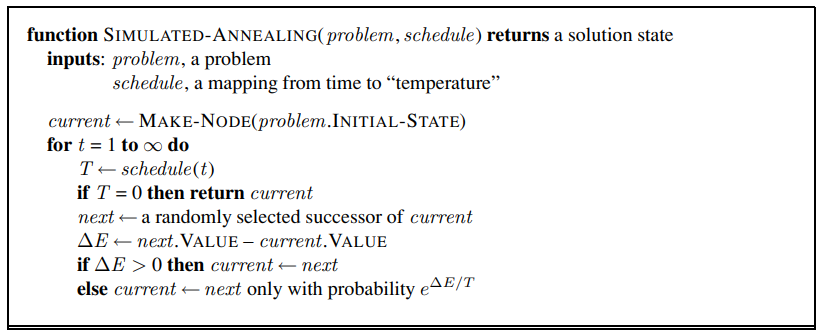
\includegraphics[]{images/annealing.png}
\end{center}
The simulated annealing algorithm is a version of stochastic hill climbing where some downhill moves are allowed. Downhill moves are accepted readily early in the annealing schedule and then less often as time goes on. The schedule input determines the value of the temperature $T$ as a function of time.\newline\newline
The innermost loop of the simulated-annealing algorithm picks a random move. If the move improves the situation, it is always accepted. Otherwise, the algorithm accepts the move with some probability less than 1. The probability decreases exponentially with the “badness” of the move, that is, the amount $\Delta E$ by which the evaluation is worsened. The probability also decreases as the “temperature” $T$ goes down: “bad” moves are more likely to be allowed at the start when $T$ is high, and they become more unlikely as $T$ decreases. If the schedule lowers $T$ slowly enough, the algorithm will find a global optimum with probability approaching 1.

\section{ Local beam search}
The local beam search algorithm keeps track of $k$ states rather than just one. It begins with $k$ randomly generated states. At each step, all the successors of all $k$ states are generated. If any one is a goal, the algorithm halts. Otherwise, it selects the $k$ best successors from the \textbf{complete} list and repeats.\newline\newline
At first sight, a local beam search with $k$ states might seem to be nothing more than running $k$ random restarts in parallel instead of in sequence. However, the two algorithms are quite different. In a random-restart search, each search process runs independently of the others. In a local beam search, useful information is passed among the parallel search threads.\newline\newline
In its simplest form, local beam search can suffer from a lack of diversity among the $k$ states—they can quickly become concentrated in a small region of the state space, making the search little more than an expensive version of hill climbing. A variant called stochastic beam search, analogous to stochastic hill climbing, helps alleviate this problem. Instead of choosing the best $k$ from the the pool of candidate successors, stochastic beam search
chooses $k$ successors at random, with the probability of choosing a given successor being an increasing function of its value.

\section{Genetic algorithms}
A \textbf{genetic algorithm} (or GA) is a variant of stochastic beam search in which successor states are generated by combining two parent states rather than by modifying a single state.\newline\newline
Like beam searches, GAs begin with a set of $k$ randomly generated states, called the \textbf{population}. Each state, or \textbf{individual}, is represented as a string over a finite alphabet, most commonly, a string of 0s and 1s. The production of the next generation of states works as follows:
\begin{enumerate}
    \item Each state is rated by the objective function, or (in GA terminology) the \textbf{fitness function}. A fitness function should return higher values for better states.

    \item for $i=1$ to $size(population)$:

    \begin{enumerate}
        \item A pair is selected at random for reproduction (the probability of being chosen for reproducing is directly proportional to the fitness score). A \textbf{crossover} point is chosen randomly from the positions in the string.

        \item A new child is generated starting from the parents according to the crossover point $c$. Basically, given $n$ the length of the representation string, the child is generated concatenating the substring of the first parent from 1 to $c$ and the substring of the second parent from $c + 1$ to $n$.

        \item Finally, the child is subject to random mutation with a small independent probability and is then added to the new population. 
    \end{enumerate}
     \item Then, the old population is updated to the new population.
    
    
\end{enumerate}


\begin{center}
    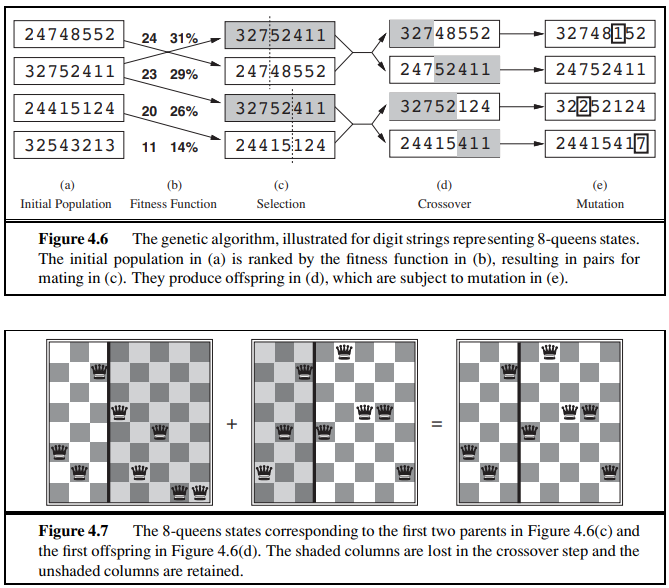
\includegraphics[]{images/GA.png}
\end{center}


\section{Continuous Spaces: Gradient Descent}
Yet none of the algorithms we have described (except for first-choice hill climbing and simulated annealing) can handle continuous state and action spaces, because they have infinite branching factors.\newline\newline
The idea is to minimize/maximize an objective function exploiting its gradient with respect to a set of parameters. The gradient vector can be interpreted as the direction and rate of fastest increase of the function. The gradient is the zero vector at a point if and only if the point is a stationary point.\\\\
This minimization problem can be solved using gradient descent. Starting from a random configuration of $\theta$, each parameter is updated in the following way:
\[\theta_{k+1} = \theta_{k} - \eta \nabla f(\theta_{k})\]
where:
\begin{itemize}
    \item $\nabla f(\theta_{k})$ is the partial derivative of the function in $\theta_{k}$.
    \item The parameter $\eta > 0$ is known as the \textit{learning rate}. 
\end{itemize}
The derivative term $\frac{\partial}{\partial \theta_{k}}f(\theta_{k})$ can be:
\begin{itemize}
    \item $\geq 0$ it means that the function is increasing, so we are decreasing $\theta_{k}$ in the \textit{right direction}.
    \item $\leq 0$ it means that the function is decreasing, so we are increasing $\theta_{k}$ in the \textit{right direction}
\end{itemize}
If $\eta$ is too small, gradient descent can be slow. Anyway, if it is too large, it can overshoot the minimum (fail to converge). 

\section{Online Search}
So far we have concentrated on agents that use \textbf{offline search} algorithms. They compute a complete solution before setting foot in the real world and then execute the solution. In contrast, when the environment is not completely observable, or it is dynamic/semidynamic, the agent needs to interact with the environment to extract information. An \textbf{online search} agent interleaves computation and action: first it takes an action, then it observes the environment and computes the next action. Online search is a necessary idea for unknown environments, where the agent does not know what states exist or what its actions do. In this state of ignorance, the agent faces an \textbf{exploration problem}.\newline\newline

\subsection{Online Search Problems}
We assume a deterministic and fully observable environment, however the agent knows only the following:
\begin{itemize}
    \item ACTIONS($s$), which returns a list of actions allowed in state $s$;

    \item The step-cost function $c(s, a, s')$, note that this cannot be used until the agent knows that $s'$ is the outcome;

    \item GOAL-TEST($s$).
\end{itemize}
If some actions are irreversible the online search might accidentally reach a \textbf{dead-end state}. In general, this is not avoidable (not even for safely explorable state spaces).
\begin{center}
    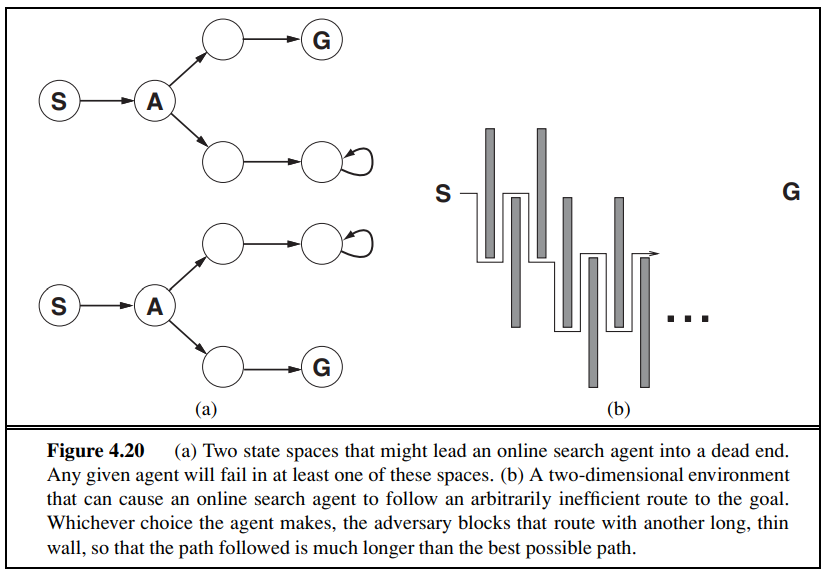
\includegraphics[scale=0.8]{images/dead-end.png}
\end{center}
Typically, the agent’s objective is to reach a goal state while minimizing cost. (Another possible objective is simply to explore the entire environment). The cost is the total path cost of the path that the agent actually travels. It is common to compare this cost with the path cost of the path the agent would follow \textit{if it knew the search space in advance}, that is, the actual shortest path (or shortest complete exploration).  In the language of online algorithms, this is called the \textbf{competitive ratio}; we would like it to be as small as possible.

\subsection{Depth-first Online Search}
After each action, an online agent receives a percept telling it what state it has reached; from this information, it can augment its map of the environment. The current map is used to decide where to go next. Offline algorithms such as A* can expand a node in one part of the space and then immediately expand a node in another part of the space, because node expansion involves simulated rather than real actions. An online algorithm, on the other hand, can discover successors only for a node that it physically occupies. To avoid traveling all the way across the tree to expand the next node, it seems better to expand nodes in a \textbf{local} order.
\newline\newline
Depth-first search has exactly this property because (except when backtracking) the next node expanded is a child of the previous node expanded.
\begin{center}
    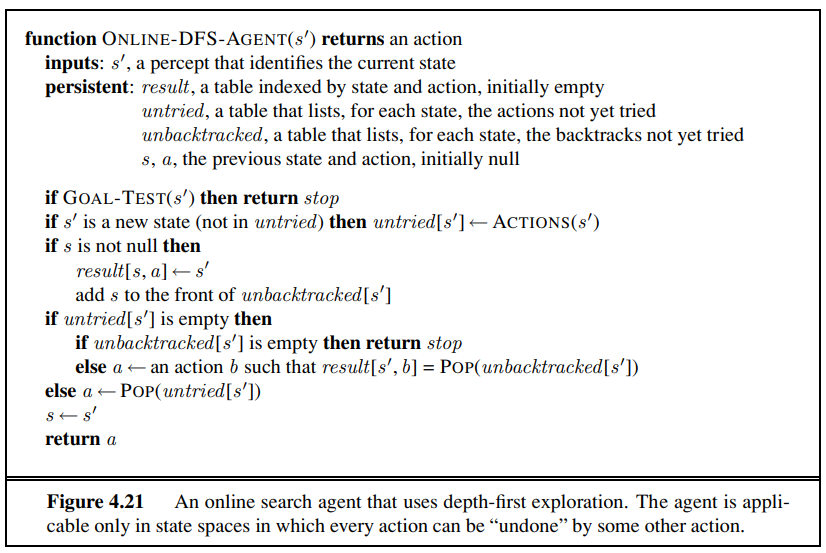
\includegraphics[]{images/online-dfs.png}
\end{center}
This agent stores its map in a table, RESULT[$s, a$], that records the state resulting from executing action $a$ in state $s$. Whenever an action from the current state has not been explored, the agent tries that action. The difficulty comes when the agent has tried all the actions in a state. In offline depth-first search, the state is simply dropped from the queue; in an online search, the agent has to backtrack physically. To achieve that, the algorithm keeps a table that lists, for each state, the predecessor states to which the agent has not yet backtracked. If the agent has run out of states to which it can backtrack, then its search is complete.

\section{Random Search}
Like depth-first search, hill-climbing search has the property of locality in its node expansions. However, random restarts cannot be used, because the agent cannot transport itself to a new state. Instead of random restarts, one might consider using a \textbf{random walk} to explore the environment. A random walk simply selects at random one of the available actions from the current state; preference can be given to actions that have not yet been tried. It is easy to prove that a random walk will eventually find a goal or complete its exploration, provided that the space is finite. On the other hand, the process can be very slow. Augmenting hill climbing with memory rather than randomness turns out to be a more effective approach.

\subsection{LRTA* Search}
The basic idea is to store a “current best estimate” $H(s)$ of the cost to reach the goal from each state that has been visited. $H(s)$ starts out being just the heuristic estimate $h(s)$ and is updated as the agent gains experience in the state space.
\begin{center}
    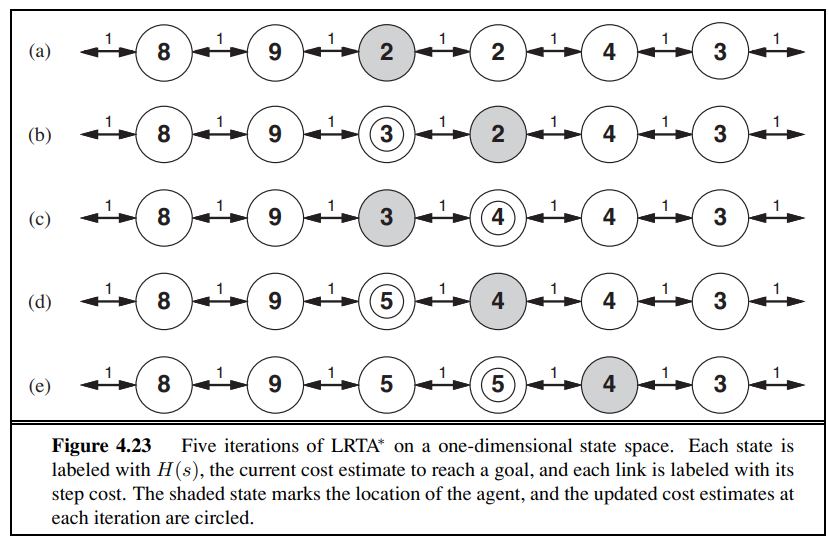
\includegraphics[scale=0.8]{images/LRTA.png}
\end{center}
The agent should follow what seems to be the best path to the goal given the current cost estimates for its neighbors.  The estimated cost to reach the goal through a neighbor $s'$ is the cost to get to $s'$ plus the estimated cost to get to a goal from there, that is, $c(s, a, s') + H(s')$. In the
example, there are two actions, with estimated costs 1+9 and 1+2, so it seems best to move right.\newline\newline
An agent implementing this scheme, which is called learning real-time A* (\textbf{LRTA*}). It builds a map of the environment in the result table. It updates the cost estimate for the state it has just left and then chooses the “apparently best” move according to its current cost estimates. One important detail is that actions that have not yet been tried in a state $s$ are always assumed to lead immediately to the goal with the least possible cost, namely $h(s)$.
\begin{center}
    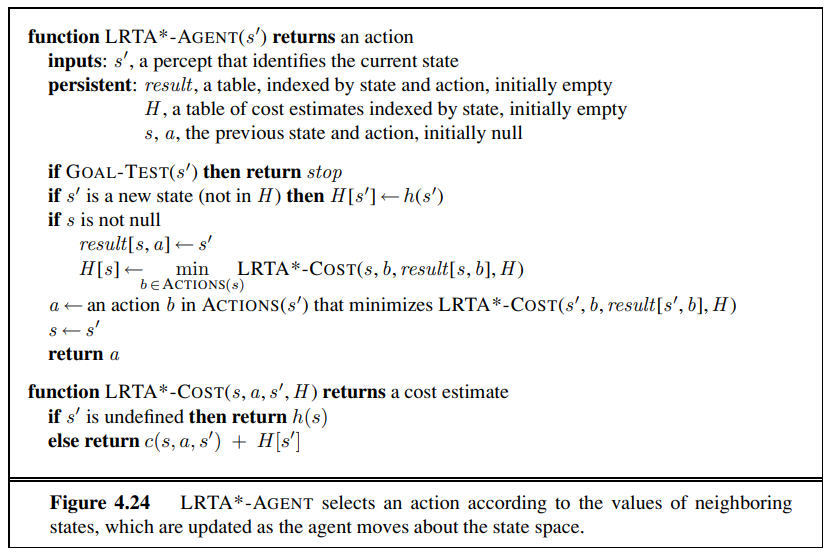
\includegraphics[scale=0.8]{images/LRTA-2.png}
\end{center}
